\documentclass[t,mathserif,10pt,aspectratio=1610]{beamer}
% option "t" means align top
% option "handout" for handout mode (each frame takes only one page)
% option "notes" to add notes pages

\setbeamertemplate{footline}[frame number]

\mode<presentation>
{
  \usetheme{bo}
}

\newcommand{\mycite}[1]{{\footnotesize [\textit{#1}]}}

\newcommand{\centergraphics}[2]{
  \begin{center}
  \includegraphics[width=#1\textwidth]{#2}
  \end{center}} % end newcommand

\newcommand{\centerboxgraphics}[2]{
  \begin{center}
  \fbox{\includegraphics[width=#1\textwidth]{#2}}
  \end{center}} % end newcommand

\newcommand\blfootnote[1]{%
  \begingroup
  \renewcommand\thefootnote{}\footnote{#1}%
  \addtocounter{footnote}{-1}%
  \endgroup
}


\newtheorem{myfact}{Fact}
\newtheorem{prop}{Proposition}
\newtheorem*{theorem*}{Theorem}
\newtheorem{question}{Question}

\DeclareMathOperator*{\E}{\mathbb{E}}


\newcommand{\kl}{\textnormal{KL}}
\newcommand{\relint}{\textnormal{relint}}
\newcommand{\tr}{\top}
\newcommand{\id}{\mathop{\mathrm{id}}}
\newcommand{\Var}{\mathop{\mathrm{Var}}}

\newcommand{\loss}{\ell}

\newcommand{\A}{\mathcal{A}}
\newcommand{\B}{\mathcal{B}}
\newcommand{\D}{\mathcal{D}}
\newcommand{\F}{\mathcal{F}}
\newcommand{\G}{\mathcal{G}}
\renewcommand{\H}{\mathcal{H}}
\newcommand{\I}{\mathcal{I}}
\newcommand{\K}{\mathcal{K}}
\renewcommand{\L}{\mathcal{L}}
\newcommand{\M}{\mathrm{M}}
\newcommand{\N}{\mathbb{N}}
\renewcommand{\O}{\mathcal{O}}
\renewcommand{\P}{\mathcal{P}}
\newcommand{\Q}{\mathcal{Q}}
\newcommand{\R}{\mathcal{R}}
\let\oldS\S % section symbol!
\newcommand{\sect}{\mbox{\oldS\hspace{-.1mm}}}
\renewcommand{\S}{\mathcal{S}}
\newcommand{\T}{\mathcal{T}}
\newcommand{\V}{\mathcal{V}}
\newcommand{\W}{\mathcal{W}}
\newcommand{\Y}{\mathcal{Y}}
\newcommand{\X}{\mathcal{X}}

\renewcommand{\vec}[1]{{\mathbf{#1}}}
\newcommand{\1}{\vec{1}}
\newcommand{\0}{\vec{0}}
\renewcommand{\b}{\vec{b}}
\newcommand{\e}{\vec{e}}
\newcommand{\g}{\vec{g}}
\renewcommand{\l}{\boldsymbol{\ell}}
\newcommand{\m}{\vec{m}}
\renewcommand{\o}{\mathit{o}}
\newcommand{\p}{\vec{p}}
\newcommand{\q}{\vec{q}}
\renewcommand{\r}{\vec{r}}
\newcommand{\s}{\vec{s}}
\renewcommand{\u}{\vec{u}}
\renewcommand{\v}{\vec{v}}
\newcommand{\w}{\vec{w}}
\newcommand{\x}{\vec{x}}
\newcommand{\y}{\vec{y}}
\newcommand{\z}{\vec{z}}

\newcommand{\convhull}{\mathsf{Conv}}
\newcommand{\conv}{\convhull}
\newcommand{\ext}{\mathrm{ext}}
\newcommand{\clo}{\mathrm{cl}}
\newcommand{\linear}{\mathsf{Lin}}
\newcommand{\affine}{\mathsf{Aff}}
\newcommand{\subgrad}[1]{d #1}
\newcommand{\subtang}[1]{d #1}
\newcommand{\subdiff}[1]{\partial #1}
\newcommand{\selsubgrad}[2]{\in \partial {#1}}%|_{#2}}
\newcommand{\toto}{\rightrightarrows}
\newcommand{\eval}{\mathsf{Eval}}
\newcommand{\nondiff}{\mathsf{nondiff}}
\newcommand{\cell}{\mathrm{cell}}
\newcommand{\lsc}{l.s.c.}
\newcommand{\dom}{\mathrm{dom}}
\newcommand{\defeq}{\doteq}%\vcentcolon=} % define equals
\newcommand{\ones}{\mathbf{1}}
\newcommand{\abs}[1]{\left\lvert #1 \right\rvert}
\newcommand{\sgn}{\mathrm{sgn}}
\newcommand{\im}{\mathop{\mathrm{im}}}
\newcommand{\spn}{\mathop{\mathrm{span}}}
\newcommand{\affspn}{\mathop{\mathrm{affinespan}}}

\newcommand{\elic}{\mathsf{elic}}
\newcommand{\elici}{\elic_\ID}
\newcommand{\iden}{\mathsf{iden}}
\newcommand{\EL}{\mathcal{E}}
\newcommand{\ID}{\mathcal{I}}
\newcommand{\ES}{\mathrm{ES}}
\newcommand{\lbar}{\underline{L}}

\def\reals{\mathbb{R}}
\def\integers{\mathbb{Z}}
\def\extreals{\mathbb{\overline{R}}}

\newcommand{\argmin}{\mathop{\mathrm{argmin}}}
\newcommand{\argmax}{\mathop{\mathrm{argmax}}}
\newcommand{\arginf}{\mathop{\mathrm{arginf}}}
\newcommand{\argsup}{\mathop{\mathrm{argsup}}}





\usepackage{adjustbox}


\title{\Large\textbf{Surrogate Regret Bounds for Polyhedral Losses}}
%\titlegraphic{
%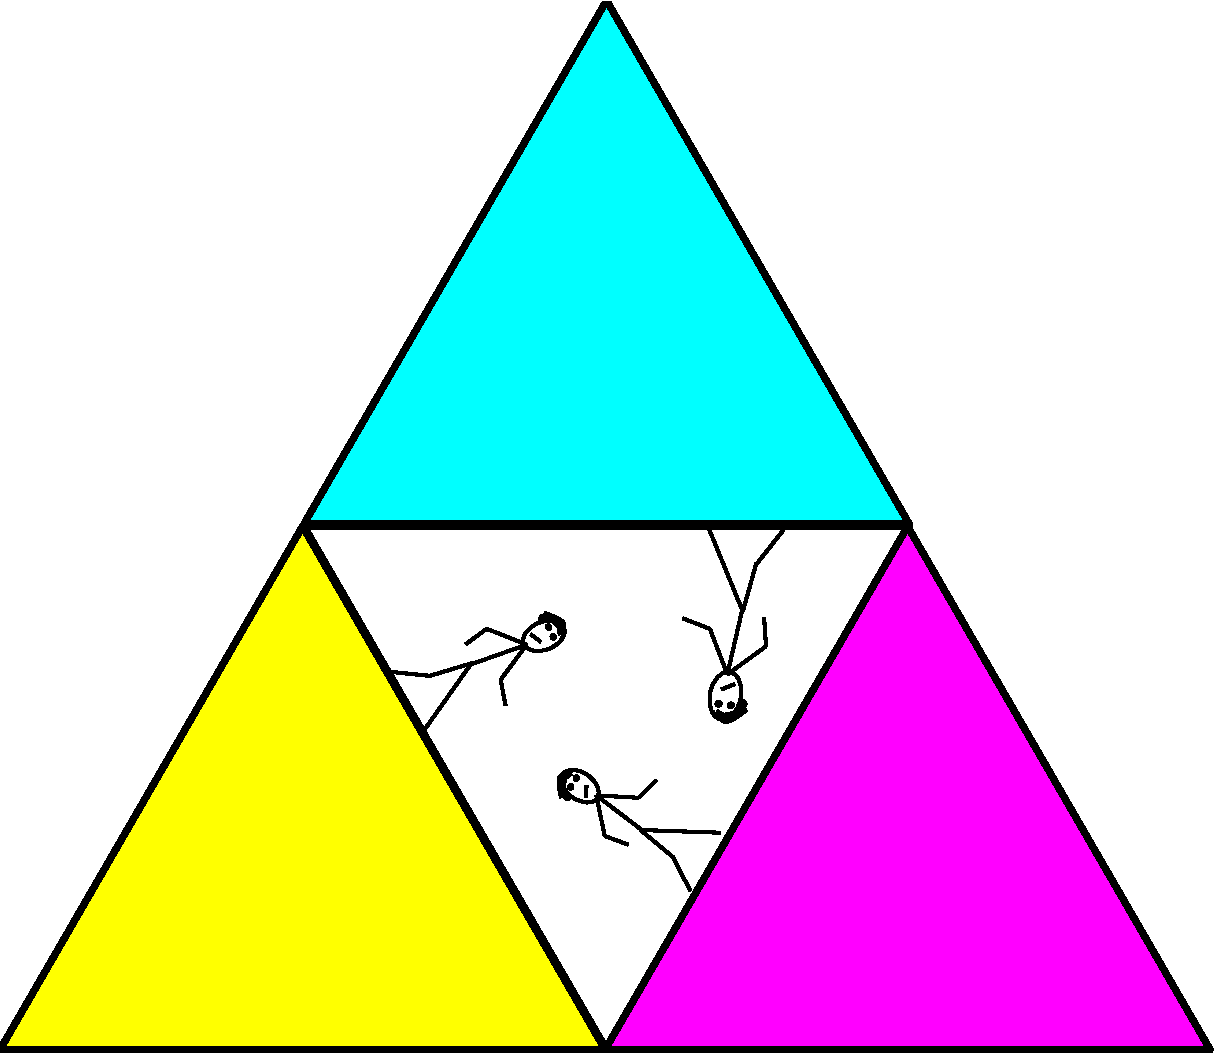
\includegraphics[width=.35\textheight]{figs/logo}
%}

\author[Bo and Raf]{{\textbf{Rafael Frongillo} and \textbf{Bo Waggoner}} \and {University of Colorado, Boulder}}
\date{\textbf{NeurIPS 2021}}

\begin{document}

%%%%%%%%%%%%%%%%%%%%%%%%%%%%%%%%%%%%%%%%%%%%%%%%%%%%%%%%%%%%%%%
\begin{frame}
  \titlepage
\end{frame}

%%%%%%%%%%%%%%%%%%%%%%%%%%%%%%%%%%%%%%%%%%%%%%%%%%%%%%%%%%%%%%
\begin{frame}{The short version}{}
  TODO: switch red and blue
  Surrogate risk minimization:
  \pause
  \begin{itemize}[<+->]
    \item Goal: optimize \blueem{discrete ``target''} loss $\ell(r,y)$  \hintright{e.g. classification, structured predictions, \dots}  \\
          \hint{$r = $ prediction in a finite set, $y = $ label}
    \item Approach: optimize \redem{continuous ``surrogate''} loss $L(u,y)$  \hintright{then ``link'' to target prediction $r = \psi(u)$} \\
          \hint{$u = $ prediction in $\reals^d$}
  \end{itemize}

  \only<3>{
    \centergraphics{0.9}{figs/hinge}
  }

  \pause
  \vskip2em
  Question: when does (quick) \redem{surrogate} convergence imply (quick) \blueem{target} convergence?  \\
  \hint{``Surrogate regret bounds'' or ``regret transfer rates''}

  \pause
  \vskip2em
  This paper: \textbf{polyhedral surrogates}  \hintright{piecewise-linear and convex}
  \begin{enumerate}[<+->]
    \item \emph{All} polyhedral surrogates have \textbf{linear} regret transfer rates!
    \item \emph{All} sufficiently ``non-polyhedral'' surrogate transfers are \textbf{quadratically slower}.
  \end{enumerate}

  \pause
  \vskip2em
  \textbf{Polyhedral:} \redem{Surrogate regret} $\leq \epsilon$ $\implies$ \blueem{target regret} $\leq O(\epsilon)$  \\
  \pause \textbf{Non-polyhedral:} Sometimes, \redem{surrogate regret} $\leq \epsilon$ yet \blueem{target regret} $\geq \Omega(\sqrt{\epsilon})$.
\end{frame}


%%%%%%%%%%%%%%%%%%%%%%%%%%%%%%%%%%%%%%%%%%%%%%%%%%%%%%%%%%%%%%
%%%%%%%%%%%%%%%%%%%%%%%%%%%%%%%%%%%%%%%%%%%%%%%%%%%%%%%%%%%%%%
%%%%%%%%%%%%%%%%%%%%%%%%%%%%%%%%%%%%%%%%%%%%%%%%%%%%%%%%%%%%%%
%%%%%%%%%%%%%%%%%%%%%%%%%%%%%%%%%%%%%%%%%%%%%%%%%%%%%%%%%%%%%%
%%%%%%%%%%%%%%%%%%%%%%%%%%%%%%%%%%%%%%%%%%%%%%%%%%%%%%%%%%%%%%
%%%%%%%%%%%%%%%%%%%%%%%%%%%%%%%%%%%%%%%%%%%%%%%%%%%%%%%%%%%%%%
%%%%%%%%%%%%%%%%%%%%%%%%%%%%%%%%%%%%%%%%%%%%%%%%%%%%%%%%%%%%%%

%%%%%%%%%%%%%%%%%%%%%%%%%%%%%%%%%%%%%%%%%%%%%%%%%%%%%%%%%%%%%%
%%%%%%%%%%%%%%%%%%%%%%%%%%%%%%%%%%%%%%%%%%%%%%%%%%%%%%%%%%%%%%
%%%%%%%%%%%%%%%%%%%%%%%%%%%%%%%%%%%%%%%%%%%%%%%%%%%%%%%%%%%%%%
%%%%%%%%%%%%%%%%%%%%%%%%%%%%%%%%%%%%%%%%%%%%%%%%%%%%%%%%%%%%%%
%%%%%%%%%%%%%%%%%%%%%%%%%%%%%%%%%%%%%%%%%%%%%%%%%%%%%%%%%%%%%%
%%%%%%%%%%%%%%%%%%%%%%%%%%%%%%%%%%%%%%%%%%%%%%%%%%%%%%%%%%%%%%

\end{document}

